\chapter{Results and Discussion}
\label{resultanddiscussion}
In this chapter the results of the conducted tests will be analysed and discussed. This is the last step in the first phase of the developement of the Artificial Eye and is shown as orange-bordered in figure \ref{ChainOpti}. Further, in this chapter the changes that were made to the Artificial Eye, based on the test results, will be explained. 

\begin{figure}[h]
\begin{center}
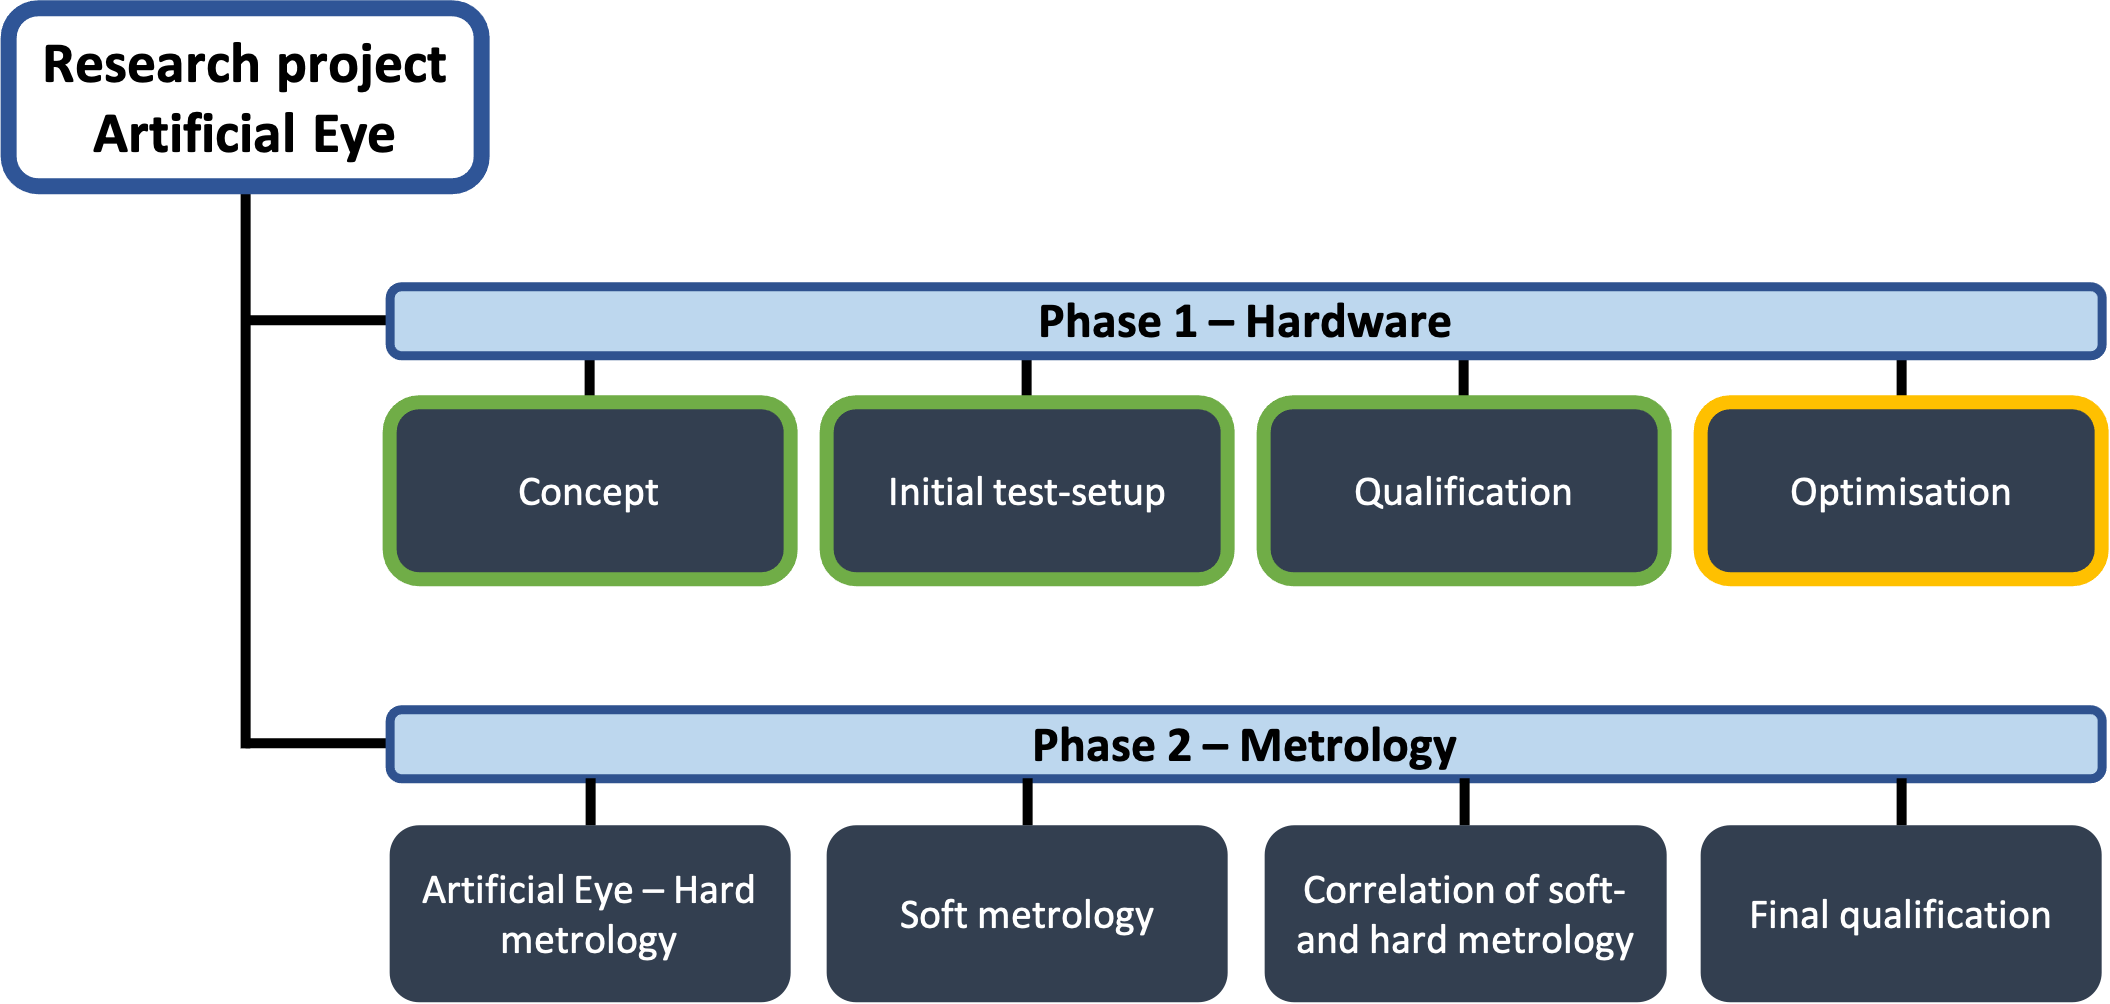
\includegraphics[width=12cm]{Pictures/ChainOpti}
\caption[Overview over the development process - Optimisation]{Overview over the development process - Optimisation}
\label{ChainOpti}
\end{center}
\end{figure}

\section{Transmission test}
This section shows the evaluation of the tests done to determine if the transmission capability of the optical system is adequate for the intended use. The key variable for the evaluation of the transmitted light was the average light intensity of each of the images captured by the four cameras. This evaluation was done with a function written in MATLAB (see Appendix \ref{appendixSoureCode}) . The function read the four images from a directory defined by the user. Next, the 12 bit pixel values (numbers from 0-4096 in increments of 1) were scaled to floating point values in a range from 0-1 (0 = black pixel, 1 = white pixel). This step was not strictly necessary, but compressed the results and made them more intuitive to evaluate. Next, the average value of all pixels for each image was calculated. The result was also a value in the range from 0-1, where 0 would represent a completely black and 1 would represent a completely white image. Based on this value, the brightness of the image could now be judged objectively. Based on the reference image, a brightness threshold of 0.3 was defined.\\
The results of the evaluation are shown in table \ref{TransmissionTable}. As one can clearly see, only the RGB camera is showing results which are higher than 0.3. With at values of 0.1439, 0.0671 and 0.0118 the colour filtered cameras are showing significantly underexposed images, already at the highest possible analog gain. Further it is important to note, that the intensity of the image captured by the blue camera, is a gratitude smaller than the values of the other images in this testing series.

\begin{table}
\begin{center}

\caption{Table with the results of the transmission evaluation}
\label{TransmissionTable}
\begin{tabular}{c|c|c|c|c}

\bfseries Analogue Gain (dB) & \bfseries RGB & \bfseries Red & \bfseries Green & \bfseries Blue
\csvreader[head to column names, separator=semicolon]{Tables/TransmissionData.csv}{}%
{\\\hline\Gain & \RGB & \Red & \Green & \Blue}

\end{tabular}
\end{center}
\end{table}

The behaviour shown above can be traced back to different causes, with the most problematic one of them being the three very narrow bandpass filters. With a bandwidth of 10 nm, the amount of light which reaches the CMOS chip of the cameras is significantly reduced. Further, the used bandpass filters have a maximum transmission rate of $\sim$50 \%. This, in combination with two 50/50 beamsplitters, reduces the maximum intensity of the light to only 12.5 \% of the initial intensity. This can be seen in figure \ref{FilterOldSpec}, which shows the spectrum that was recorded during the tests as well as the the transmission functions of the colour filters. Looking a the graph of the spectrum and the filter characteristics, it also becomes obvious why the blue camera picked up less light than the red and green cameras. The light source which was used in order to illuminate the test plate, has very warm light colour (less blue and more red and green parts in the spectrum). Another interesting observation is, that the RGB camera also shows underexposed pictures for gain values smaller than 43 dB. Because the RGB camera has, besides the Bayer pattern, no additional filters, this had to be caused by other components in the optical system. As previously mentioned, the beamsplitters already reduce the incoming light by 75 \%. But another factor determining the amount of light entering the optical system is the lens. With a focal length of 75 mm and an entrance pupil diameter of 25.5 mm, the current lens has a fairly small field of view (7 mm x 5 mm at a distance of 200 mm) and can not pick up enough light.


\begin{figure}
\begin{center}
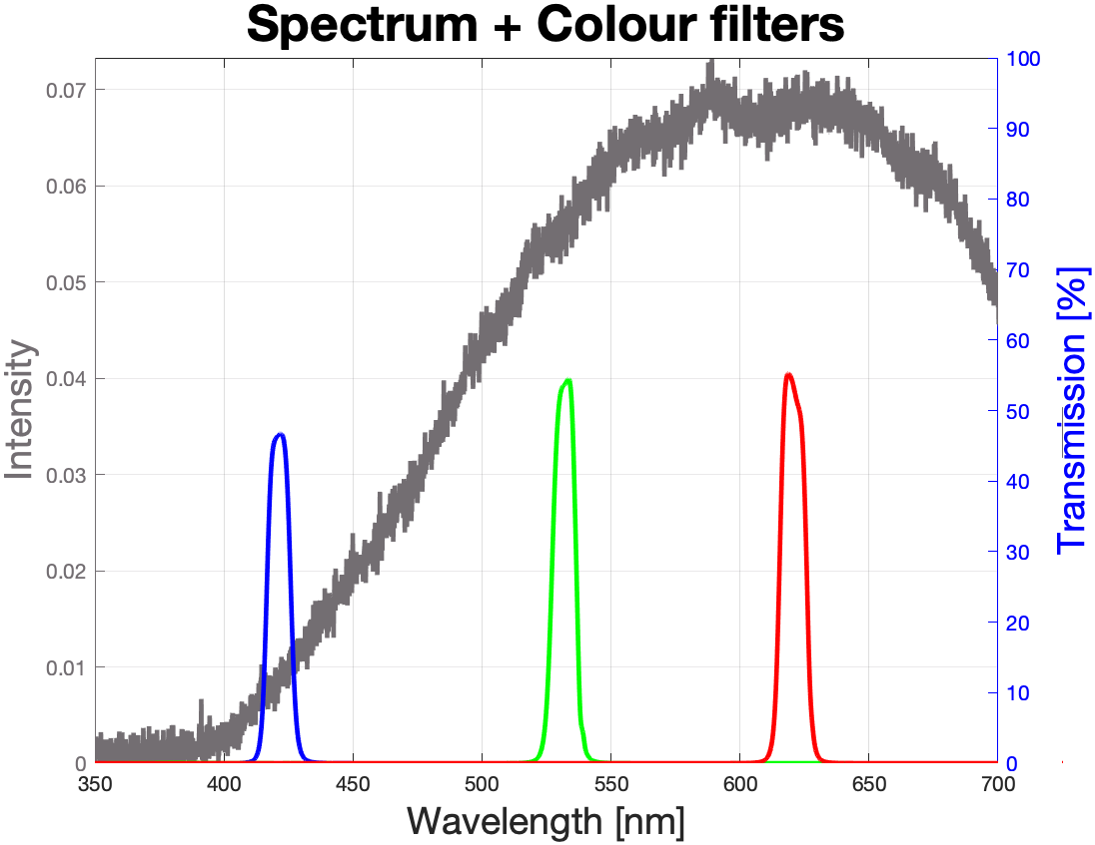
\includegraphics[width=12cm]{Pictures/SpectrumFilters}
\caption[Graph showing the spectrum of the used light source and the transmission of the colour filters]{Graph showing the spectrum of the used light source and the transmission of the colour filters}
\label{FilterOldSpec}
\end{center}
\end{figure}

\subsection{Optimisation}
In order to ensure that the system is usable under normal daylight conditions, two important changes were made to the optical system of the Artificial Eye. 
\subsubsection{Colour filter design}
The old colour filter design consisted of three bandpass filters with a bandwidth (FWHM) of 10 nm. The maximum transmission rate of the old filters was $\sim$50 \%. In order to increase the intensity of light on the monochromatic cameras three new colour filters have been selected. For the new filters, the bandwidth had been increased to 50 nm and the maximum transmission rate was increased to $\sim$98 \%. Because it was not possible to find a supplier which offered a bandpass filter with the previously mentioned characteristics, the new bandpass filters were constructed by combining a longpass filter and a shortpass filter. Figure \ref{FilterComp} shows the transmission function of both, the old and the new filters for comparison.

\begin{figure}
\begin{center}
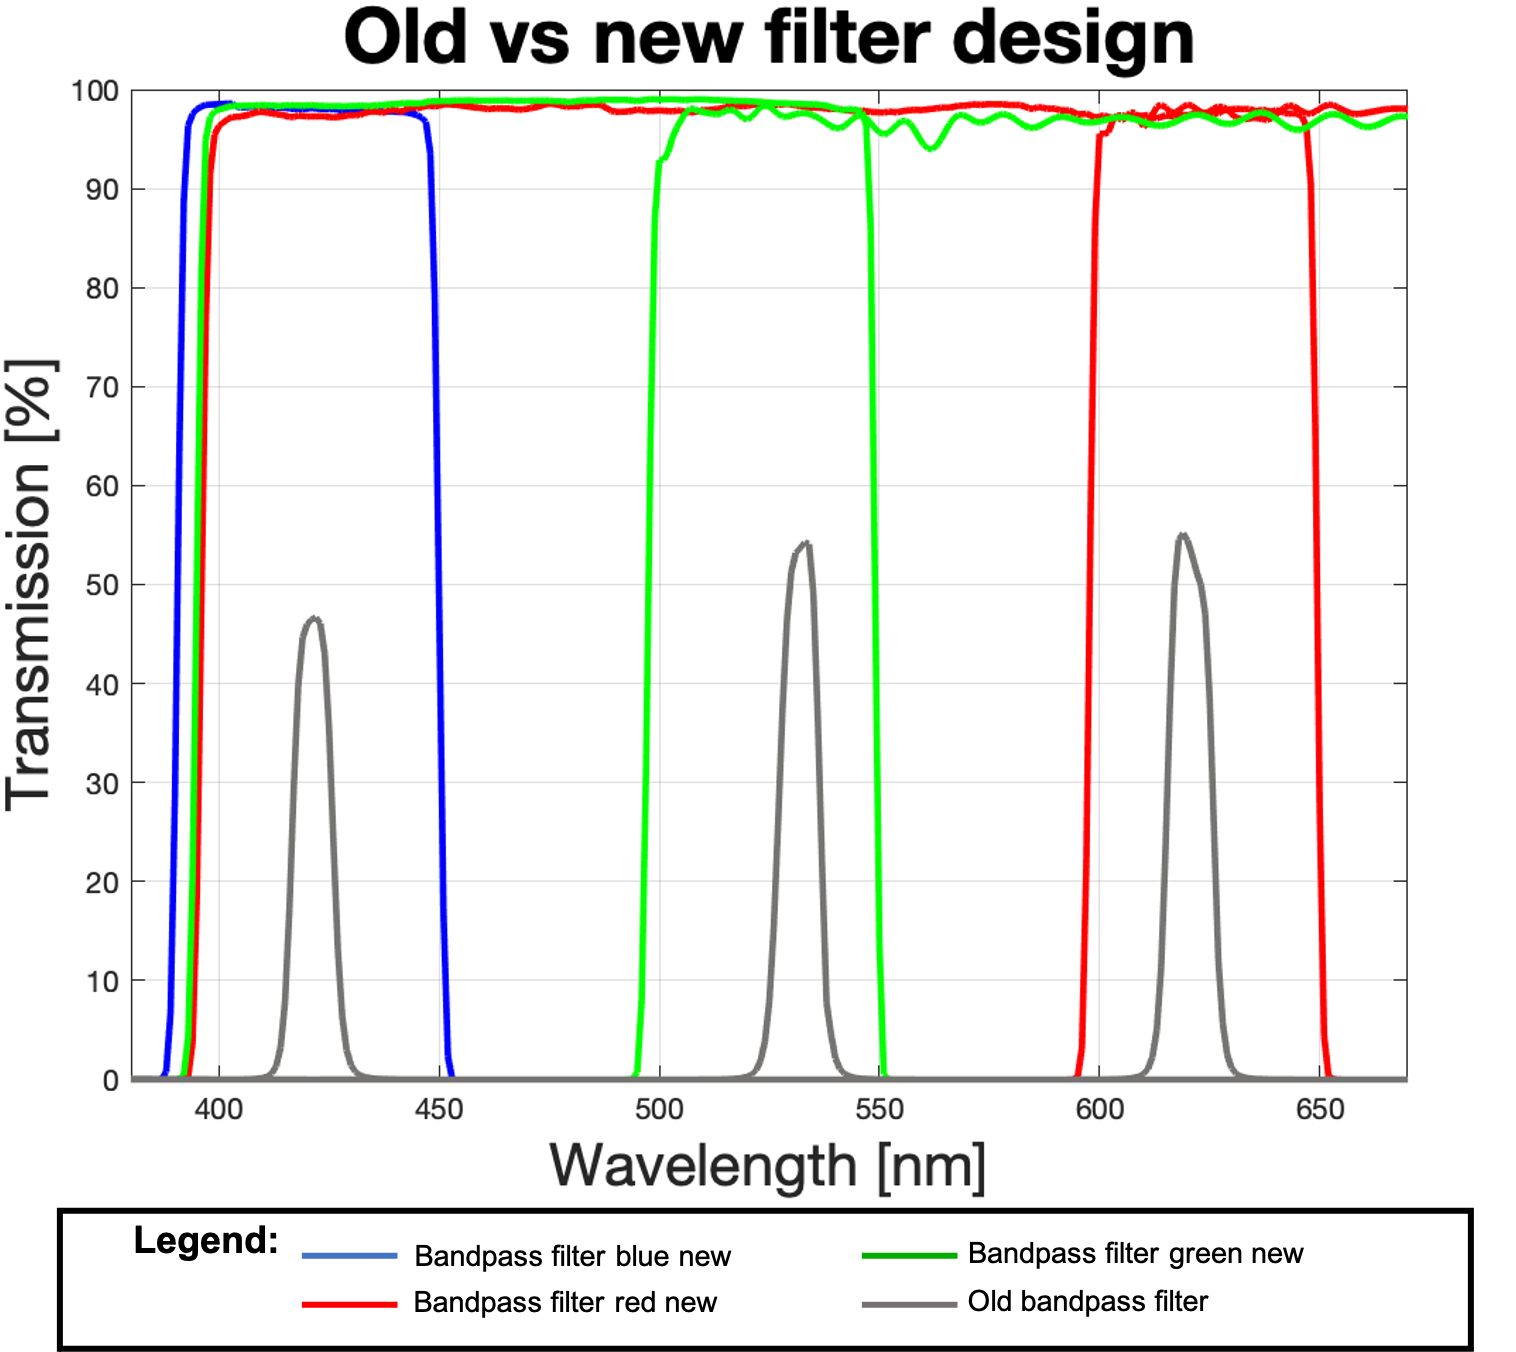
\includegraphics[width=12cm]{Pictures/AMOLEDSpectrumFilter}
\caption[Graph with the comparison of the new and old filter design]{Graph with the comparison of the new and old filter design}
\label{FilterComp}
\end{center}
\end{figure}

\subsubsection{Lens}
To further improve the image quality of the camera system, the lens of the Artificial Eye was changed. As a new lens, the zoom lens MVL7000 by Thorlabs was selected. It offers an adjustable focal distance from 18-108 mm and has a maximum entrance pupil of 43.2 mm. This not only enables the system to pick up more light, but also allows some adjustability for the field of view.\\

By changing both, the colour filter as well as the lens of the Artificial Eye, the imaging capabilities of the system increased drastically. Under the same lighting conditions, used in the initial testing series, it was now possible to capture images with an average intensity $>$0.3 using a gain value of 20 dB for the RGB camera, 27.3 dB for the red camera, 33.8 dB for the green camera and 41 dB for blue camera.

\begin{figure}
\begin{center}
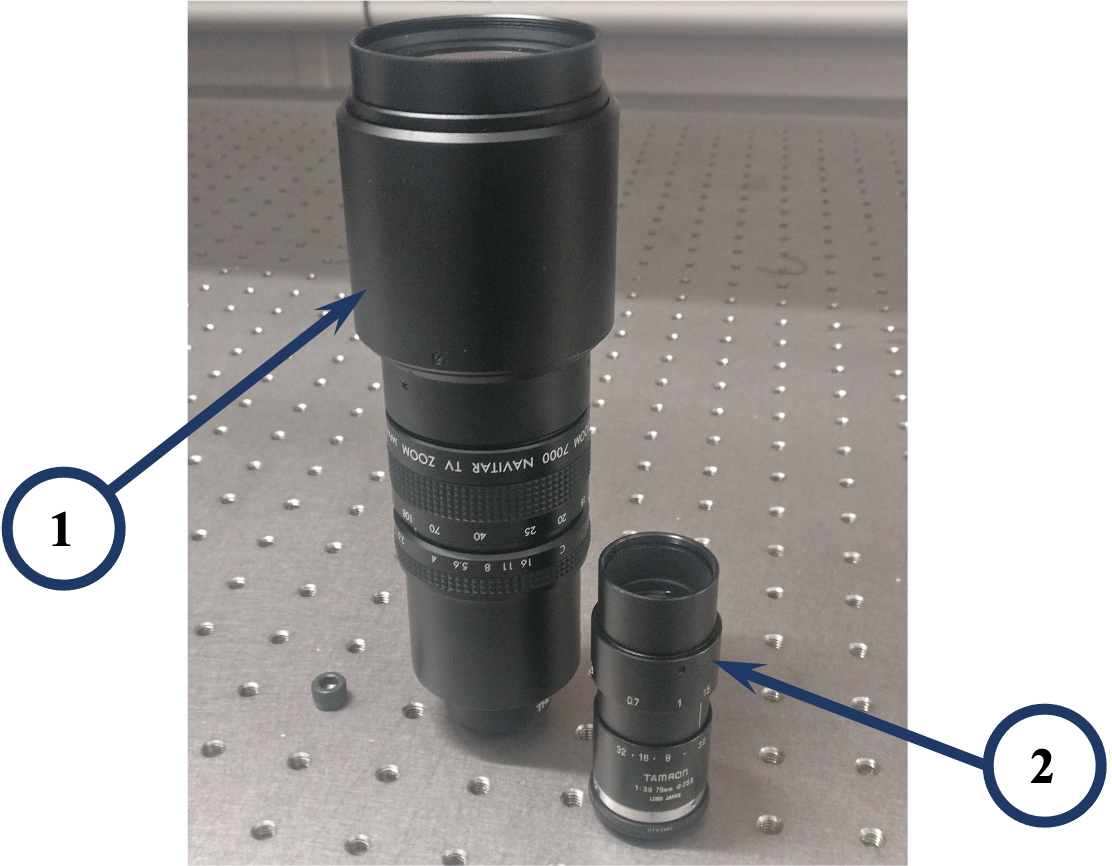
\includegraphics[width=12cm]{Pictures/LensComp}
\caption[Picture with the new and old lens side by side]{Picture with the new and old lens side by side: 1 - New zoom machine vision lens, 2 - Old fixed focal length machine vision lens}
\label{LensComp}
\end{center}
\end{figure}






\section{Focus test}
This section will show the evaluation and the results of the data, collected during the focus tests. Further, the optimisations made to the optical system of the Artificial Eye will be discussed.\\
The data collected during the focus tests consisted of an absolut position in X, Y, Z indicating the focal point of each of the four cameras. To show the differences between the cameras, the RGB camera was selected as a reference. Now the positional difference for the point, where the other cameras have been in focus, was calculated relatively to the position of the RGB camera. Both, the absolute positions (X, Y, Z) and the relative positions (X', Y', Z') are shown in \ref{FocusTable}. This data clearly shows a signifiant offset in focus (Z direction) between the cameras. In the X and Y direction (point of view) only minor differences were visible. However, it is important to notice, the relative position difference in Z is equal for all three monochromatic cameras. This indicates, that the three monochromatic cameras already share the same focal point. This way either the three monochromatic cameras or the RGB camera can be focussed and acquire sharp images. This effect also showed up in the images the system acquired to this point (see figure \ref{Fov_Foc}). Indicated by the results of this test, the unequal focal point between the cameras was caused by the unequal length of the path that the incoming light has to take from the lens to the camera. The unequal length was caused by the beamsplitter assembly, as well as the lens tubes, which were used to mount the colour filters in front of the monochromatic cameras.

\begin{table}
\begin{center}

\caption{Table with the absolute and relative position date of the camera focal point}
\label{FocusTable}
\begin{tabular}{c|c|c|c|c|c|c}

\bfseries Camera & \bfseries X [mm] & \bfseries Y [mm] & \bfseries Z [mm] & \bfseries X' [mm] & \bfseries Y' [mm] & \bfseries Z' [mm]

\csvreader[head to column names, separator=semicolon]{Tables/FocusAbs.csv}{}%
{\\\hline\C & \X & \Y & \Z & \x & \y & \z}


\end{tabular}
\end{center}
\end{table}

\begin{figure}
\begin{center}
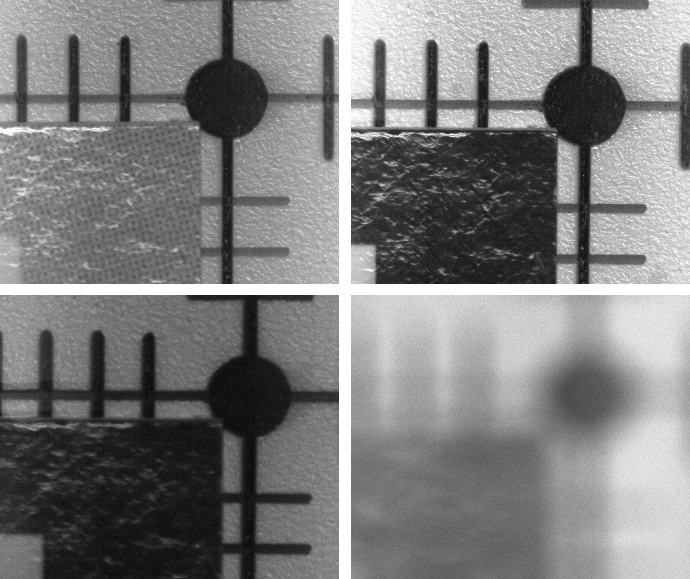
\includegraphics[width=12cm]{Pictures/FovFoc}
\caption[Camera pictures of the field of view and Focus Tests]{Camera pictures of the Field of View and Focus Tests: Top left - Pol. Red, Top right - Pol. Green, Bottom left - Pol. Blue, Bottom right - RGB}
\label{Fov_Foc}
\end{center}
\end{figure}


\subsection{Optimisation}
As mentioned previously, it is very important, that all cameras in the optical system share the same focal point. In order to adjust the focus for each of the cameras separately the threaded spacers used to mount the cameras to the beamsplitter assembly, could be screwed in or out to decrease/increase the distance to the lens. Because the pitch of threads on the spacers is very low it can only be used to make small adjustments and was not enough in this case. To equalise the distance from the lens to the cameras the assembly of the beamsplitters need to be changed. As shown in figure \ref{NewAssembly}, by mounting a beamsplitter with the fibre-coupler of the spectrometer as a first device after the lens, it was possible to equalise the length of the path of the light for all three cameras. This has the side effect that the amount of light passed to the cameras is halved. However, due to the new lens and colour filter design, the intensity of the light was still sufficient after this change. In addition to the rearrangement of the beamsplitters, an empty lens tube was added in front of the RGB camera. After the mentioned changes, all four cameras now shared the same focal point.\\
The small deviations in X and Y could be calibrated by loosening the screws, which hold the cameras to the backplate. The play in the threads of the spacer then allowed for some play in both horizontal directions. For the X direction the camera could just be carefully pushed into place. However, for the Y direction thin 0.05 mm and 0.1 mm brass shim stock was needed  in between the camera and the backplate, in order to correct for the misalignment. 

\begin{figure}
\begin{center}
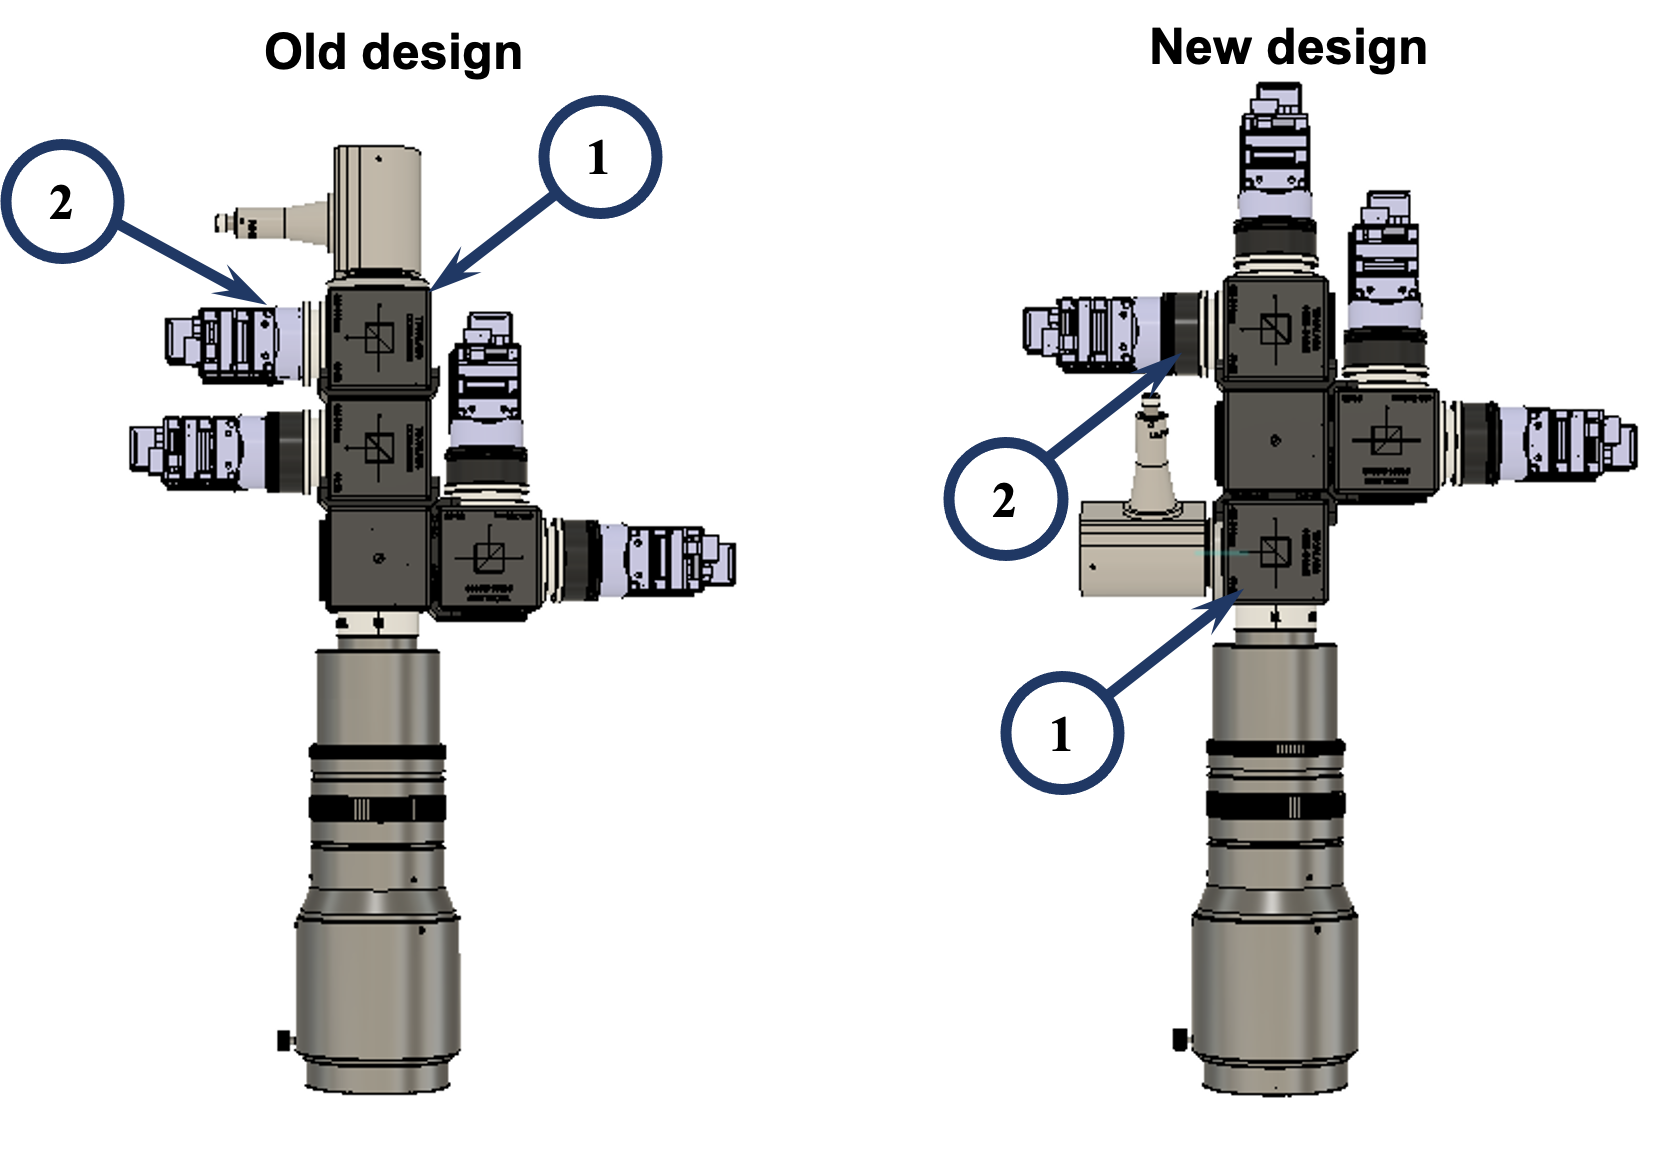
\includegraphics[width=12cm]{Pictures/NewAssembly}
\caption[Picture of the new vs. the old design of the beamsplitter assembly]{Picture of the new vs. the old design of the beamsplitter assembly}
\label{NewAssembly}
\end{center}
\end{figure}








\section{Resolution}
This section will explain the process evaluating the maximum resolution of the Artificial Eye. In order find the resolution limitations of the optical system of the Artificial Eye, a picture of every section of the resolution test plate was taken. The evaluation of these pictures was straight forward. The visible sections of the test plate on each of the images, was inspected and determined, if the small structures were still recognisable. For the bigger FOV, the structures were recognisable as separated lines, down to a spacing of 100 $\mu$m. With the smaller FOV (zoomed in) it was possible to see structures with 80 $\mu$m. The two pictures, with the maximum resolution for the big FOV and the small FOV are shown in figure \ref{ResuRes}. Further it is important to note that in order to evaluate the images correctly, it was essential to zoom into the areas of interest. This way the resolution of the computer monitor was no longer the limiting factor of the resolution of the displayed image.\\
Because the result of this test was already better than the specification of 200 $\mu$m at a distance of 700mm, no changes needed to be made to the optical system.

\begin{figure}
\begin{center}
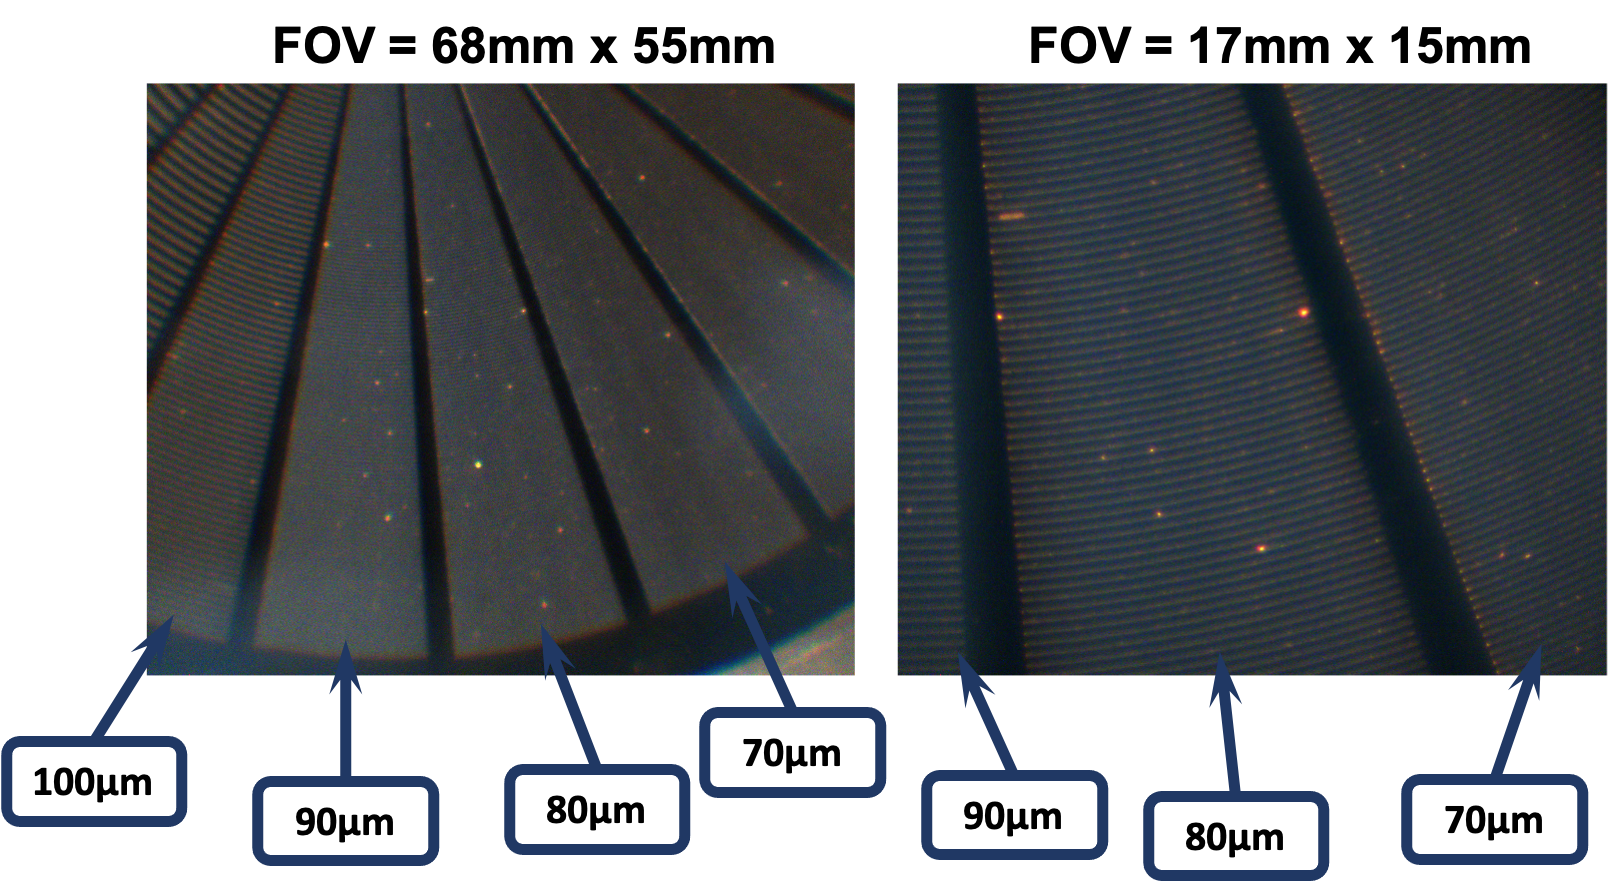
\includegraphics[width=12cm]{Pictures/ResulutionResult}
\caption[Picture of the maximum resolution of the system]{Picture of the maximum resolution of the system: Left - High FOV, Right - Low FOV}
\label{ResuRes}
\end{center}
\end{figure}












